\documentclass[11pt]{article}
\usepackage[a4paper,margin=2cm]{geometry}
\usepackage[T1]{fontenc}
\usepackage{lmodern}
\usepackage{graphicx}
\usepackage{booktabs}
\usepackage{amsmath,amssymb}
\usepackage{array}
\usepackage{caption}
\usepackage{adjustbox}
\usepackage[table]{xcolor}
\usepackage[hidelinks]{hyperref}
\captionsetup{font=small,labelfont=bf}
\captionsetup[table]{labelformat=empty}
\captionsetup[figure]{labelformat=empty}
\graphicspath{{figures/}}
\setlength{\emergencystretch}{3em}
\newcommand{\ci}[2]{[#1,\,#2]}
\newcommand{\sd}{\textsc{FileInfo}}

\newcommand{\POWERREPS}{200}\newcommand{\POWERNULL}{200}

\title{Supplementary Information\\ Discrete or graded? A confound-controlled re-analysis of clustering in Egyptian fruit bat social calls}
\author{Ninad Rai [affiliation to be added]}
\date{}

\begin{document}
\maketitle
\noindent\textbf{Abbreviations.} AUC, area under the receiver-operating-characteristic curve; ARI, adjusted Rand index; AVES, a pretrained animal-vocalisation encoder; CI, confidence interval; FCM, fuzzy c-means; FPC, fuzzy partition coefficient; HDBSCAN, hierarchical density-based clustering; MFCC, mel-frequency cepstral coefficients; NMI, normalised mutual information; PC, principal component; PS, prediction strength; SD, standard deviation; SNR, signal-to-noise ratio; UMAP, uniform manifold approximation and projection; VAE, variational autoencoder. Unless stated, the resampled or held-out unit is the bat (individual), and every interval resamples whole bats. Machine-readable results are provided as Supplementary Data files SD1--SD7 (Section~11).
\tableofcontents

\section*{S0 Extended methods}\addcontentsline{toc}{section}{S0 Extended methods}
This section gives the detail that Section~3 of the main text condenses; nothing in it changes a result.

\begin{table}[htbp]\centering\small
\caption{\textbf{Table S0.} Reproduction of the July analysis from audio (3,897 rows, 2,360 distinct annotation rows): original and reproduced values. FPC, fuzzy partition coefficient; ARI, adjusted Rand index; $|r|$, absolute correlation of the first five principal components with the saved array.}
\begin{tabular}{lcc}
\toprule
 & original & reproduced \\
\midrule
$|r|$ with saved PC1--PC5 & --- & 1.000 \\
FPC, $c=2$ & 0.5786 & 0.5786 \\
Xie--Beni & 1.2498 & 1.2496 \\
Silhouette & 0.2195 & 0.2195 \\
Cluster sizes & 1,860 / 2,037 & 1,860 / 2,037 \\
ARI vs.\ original labels & --- & 1.000 \\
Duration, cluster 0 / 1 (s) & 1.966 / 1.314 & 1.966 / 1.314 \\
Point-biserial $r$ (duration) & $-0.422$ & $-0.4223$ \\
\bottomrule
\end{tabular}
\end{table}

\paragraph{Number of bats in each analysis.} The corpus has 41 bats with positive emitter codes, all present in the 41,116-file discovery sample; with the unknown-emitter code 0 this gives the 42 emitter groups mentioned in the main text (negative codes are assigned to the absolute value of the code). The emitter-identification analyses require at least 30 files (or syllables) per bat in the analysed set, which removes bat~118 (23 files) from the file-level analyses and different bats from the smaller sets (Table~S0b). This criterion does not exclude bats from the cluster, context or Isolation analyses.

\begin{table}[htbp]\centering\scriptsize
\caption{\textbf{Table S0b.} Number of bats and the eligibility criterion in each analysis.}
\begin{tabular}{p{6.6cm}cp{6.4cm}}
\toprule
analysis (units) & bats & criterion \\
\midrule
whole corpus, 87,986 annotated files & 41 & emitter code $>0$ \\
discovery sample, 41,116 files & 41 & emitter code $>0$ (18,450 files); 42 groups with the unknown-emitter code \\
file-level emitter identification (Tables S3), 18,427 files & 40 & at least 30 files; bat 118 (23 files) excluded \\
first development set, 15,992 files & 36 & at least 30 files in that set \\
syllable-level emitter identification, 30,000 syllables & 36 & at least 30 sampled syllables \\
VAE comparison, 13,510 syllables of the 21 unseen bats & 18 & at least 30 syllables in the test half \\
replication and completion samples, each & 33 & emitter code $>0$ in that sample (all also in the discovery sample) \\
pups with known birth dates (age windows, per-pup analyses) & 20 & birth date available; 15 pups have enough files for a per-pup AUC \\
\bottomrule
\end{tabular}
\end{table}

\paragraph{Dataset A, annotation fields.} For every annotated file the annotation table lists the file, the emitter and addressee, the context, the actions of both animals before and after the call, and the start and end sample of the annotated span. The meaning of each column was checked in the dataset's metadata document before use. Emitter code 0 means that the emitter is unknown; a negative code means that the interacting pair was recognised but their roles are in doubt, so the code identifies either the emitter or the addressee. Audio was streamed from the remote archives with HTTP range requests, and no audio was stored.

\paragraph{The 19 representations.} Whole-span and voiced 1,408 statistics; whole-span and voiced MFCC statistics; syllable shape; syllable MFCC means; syllable scalar descriptors; the VAE latent space and its linear baseline; the microphone and piezo sensors of Dataset B; and the eight AVES variants (two models $\times$ whole span or voiced $\times$ plain downsampling or time expansion).

\paragraph{Features.} \emph{Whole-span:} a 128-band mel spectrogram ($n_\mathrm{fft}=2048$, hop 512, 2--125\,kHz, power in decibels; librosa), first and second temporal deltas, and per-band mean, standard deviation, skewness, kurtosis, minimum, maximum and range, giving 1,408 features over all frames of the annotated span; the decibel reference is not stated in the original, so three variants were compared. \emph{Voiced-frame:} the same statistics over frames whose centre lies inside a \sd{} voiced segment (deltas computed on the full span before masking), 20 MFCCs with deltas (120 statistics) for whole-span and voiced frames, and per file the silence fraction, SNR, noise floor, clipping fraction, voiced duration and number of voiced segments. \emph{Syllable:} for each of 141,815 voiced segments of at least 3 frames: duration, SNR, level, spectral descriptors, 19 MFCC means, and a duration- and level-free \emph{shape} (log-mel pooled to 32 bands, mean level removed, resampled to 16 time bins: 512 values); analyses used 30,000 random segments. Features were standardised and reduced to 50 principal components fitted on the analysed set (on the discovery set for the out-of-sample sets); all stochastic steps used seed 42.

\paragraph{Learned and pretrained embeddings.} The VAE (MLP 512--256--128--8, Gaussian likelihood, KL weight 0.1 or 1, 60 epochs) was trained on the syllable shapes of 21 randomly chosen bats (16,490 syllables) and applied to the 13,510 syllables of the other 21; the linear baseline used the first eight principal components of the training half. AVES embeddings (models \texttt{aves-base-bio} and \texttt{aves-base-all}; 768-d mean of the last layer; weights loaded with \texttt{weights\_only}) were extracted for 1,000 files in four variants: plain 16\,kHz downsampling or 2$\times$ time expansion (calls have a median spectral centroid of 11.4\,kHz and plain downsampling keeps only content below 8\,kHz), for the whole span or the voiced frames only.

\paragraph{Clustering algorithms.} Fifteen algorithms (26 variants) were run on the 19 representations, each on a seeded 6,000-point subsample (all points for the 1,000-file sets): centroid and model-based (k-means; FCM with $m=2$, tolerance 0.005 and 20 restarts for the reproduction of the original analysis and the confound audit, 5 in the one-cluster-allowed battery, the method comparison and the re-tests on unseen files, and 3 in the all-algorithm comparison, the power analysis and the preprocessing sensitivity analysis; Gaussian mixtures with spherical, diagonal, tied and full covariance, $k=1$--6, BIC and ICL; a Bayesian mixture with a Dirichlet-process prior; k-medoids), hierarchical (Ward, average, complete and single linkage), graph and spectral (spectral clustering with a 15-nearest-neighbour affinity; Louvain and Leiden community detection on the 15-NN graph at resolutions 1.0 and 0.1), density- and mode-based (DBSCAN at three radii; OPTICS; HDBSCAN with minimum sizes 25 and 100; mean-shift), and others (BIRCH; affinity propagation; a $3\times3$ self-organising map). Recorded per configuration: number of clusters (and of clusters holding at least 1\% of the points), noise share, silhouette of the non-noise points (3,000-point subsample), NMI with recording channel and with silence-fraction quintile, and wall-clock time.

\paragraph{Tests that allow a single cluster, nulls and power.} All resample bats, not calls; definitions are in Table~S1. The Gaussian-copula null preserves each component's empirical marginal and the rank-correlation matrix; the session-mean null simulates residuals about channel$\times$month means from a copula and adds the means back; each comparison uses 50--100 simulated datasets, and permutation $p$-values are reported as $p<1/(B+1)$ when no null replicate reaches the observed value. A simulated control with the original matrix's variance spectrum (four unimodal families, including a curved one-dimensional continuum) evaluated whether validity indices can pick $c=2$ for one population. For the power analysis, a two-type mixture was spiked into the session-mean null of the voiced file-level features and of the syllable shapes (templates of 6,000 rows) and the battery was run with reduced settings (3 FCM restarts, 10 train/test splits, 20 bootstraps). The real-data battery of Tables~S1a--S1c uses heavier settings (5 FCM restarts, 20 splits, 50 bootstraps), so the power thresholds are not numerically comparable with those tables; the same reduced pipeline was applied to the null and to the spiked data.

\paragraph{UMAP pipeline and cluster characterisation.} UMAP and HDBSCAN were additionally run with 15 and 100 neighbours and under 8 bat bootstraps, on the real data without the resulting small cluster (or without all Isolation-context files), and on the nulls named in Section~3.5 of the main text. Clusters were characterised by recording covariates (AUC; bias-corrected Cram\'er's $V$ after Bergsma), context, a within-channel$\times$month permutation of the cluster--context association, and a linear discriminant axis learned on the cluster labels of one random half of the bats and projected on the other half (standardised separation $d'$, dip test).

\paragraph{Supervised separability.} The balanced logistic regression ($C=0.5$) used the 50 components with folds blocked by bat (five folds): AUC with bat-level bootstrap intervals, $d'$ of the out-of-fold scores, and dip tests of the pooled and of the non-Isolation scores. Repetitions: within pups only, within channel$\times$month strata, per pup, without the unknown-emitter group, within pup-age windows (ages from the dataset's birth dates), with each channel or treatment held out in turn, and for syllables, the VAE and AVES.

\paragraph{Confound audit, mixed models and identity.} The cluster label was related to continuous covariates (AUC) and categorical covariates (Cram\'er's $V$) with bat-level bootstrap intervals; recording variables alone predicted the label with logistic regression with folds blocked by bat. The association of context with the label was tested within channel$\times$month strata by permutation. Mixed models used the logit of cluster membership with crossed random intercepts for bat and stratum (likelihood-ratio tests; repeatability with bat-level bootstrap). Emitter identification (positive codes, bats with at least 30 files) used multinomial logistic regression with random, day-, month-, archive- and channel-blocked folds, balanced accuracy and a permutation null (labels shuffled within channel$\times$month strata); channel normalisation (per-channel mean, per-channel standardisation, per-channel$\times$month mean; no labels used) was tested as a remedy; within-channel identification used day-blocked folds; pair-coded files were scored by the probability assigned to the two recognised participants against a within-stratum shuffle.

\section{Extended tests of cluster structure}
\paragraph{Statistics and how they are read.} Table~S1 defines each statistic, the null model it is compared with and the interpretation rule used in the main text. Tables~S1a and S1b give the observed values and null means; Table~S1c gives the position of each observed value in the null distribution as an empirical one-sided count. The comparisons are descriptive: no significance threshold or multiplicity correction is applied, and a higher observed value is read as cluster-like structure only when it exceeds the null distribution. Observed values of the one-cluster-allowed battery are given for the original matrix, the whole-span, voiced and voiced-MFCC features of the 15,992-file development set, 30,000 syllable shapes, the VAE latent space and its 8-PC baseline (unseen bats), and both sensors of Dataset B.

\begin{table}[htbp]\centering\scriptsize
\caption{\textbf{Table S1.} Statistics of the one-cluster-allowed battery: what each measures as implemented, the null it is compared with, and the interpretation rule. Both nulls have the same data size, number of bats and component marginals as the observed data and contain no discrete clusters: \emph{Gaussian copula} (marginals and rank correlations kept) and \emph{session mean} (copula residuals around channel$\times$month means, means added back). Empirical one-sided $p=(1+k)/(N+1)$ with $k$ = number of null replicates at least as large as the observed value (Table S1c).}
\begin{adjustbox}{max width=\linewidth}
\begin{tabular}{p{2.2cm}p{5.9cm}p{3.0cm}p{5.4cm}}
\toprule
statistic & what it measures & null comparison & interpretation \\
\midrule
Prediction strength (PS), $k=2$ & Bats are split into two balanced halves (20 splits, both directions). $k$-means is fitted to each half; its centroids assign the other half, and the share of test-pairs that are in the same test cluster and are also co-assigned is computed for each cluster (minimum over the two clusters) & Copula and session-mean nulls; observed value, null mean, position (Table S1c) & Reproducibility of the partition across individuals; structure is supported only if PS is at or above the conventional 0.8 reference and is not below the null; a value below the null means a less stable partition than data without structure \\
Bootstrap Jaccard stability & $k$-means partition of all rows; 50 resamples of whole bats; for each original cluster the best Jaccard overlap with a cluster of the resample; mean & same nulls & High stability alone does not prove clusters, because structureless data can also give high values; the observed value is read relative to the null \\
Silhouette, $c=2$ & Mean silhouette width of the hard labels of the two-cluster FCM partition & same nulls & Higher = better separated, read against the null baseline (structureless data give positive silhouettes); an excess that follows duration or SNR is not evidence of discrete call types (main text) \\
FPC excess & FPC $-1/c$ at $c=2$: departure from the value 0.5 of a single cluster & same nulls & $0$ = the one-cluster solution; a positive excess alone is insufficient evidence, because non-Gaussian structureless data also give positive excess \\
Split-sample Hartigan dip & Dip statistic of the held-out half projected on the axis between the two $k$-means centroids of the training half; mean over 20 splits; median dip $p$ (syllables or files treated as independent, hence optimistic) & same nulls & Tests unimodality along the tested axis only; limited power for minorities below 10\% (Section~2), so it can exclude a valley but not a rare group \\
Gap statistic & Mean log within-cluster dispersion of 10 uniform reference datasets minus that of the data, for $k=1$--6; $k$ is the smallest value with gap$(k)\ge$ gap$(k+1)-s_{k+1}$; the difference gap(2)$-$gap(1) is recorded & same nulls & Chose the maximum $k$ for data and nulls alike; not used for any conclusion \\
\bottomrule
\end{tabular}
\end{adjustbox}
\end{table}

\begin{table}[htbp]\centering\scriptsize
\caption{\textbf{Table S1a.} Prediction strength (PS; bat-level 95\% interval in brackets) and bootstrap Jaccard stability at $k=2$ (definitions in Table S1): observed value, mean of the Gaussian-copula null (cop.) and of the session-mean null (ses.), each over 50--100 simulated datasets. Higher = more stable. Representations: file-level features of the 15,992-file development set unless stated; unseen bats = the 21 bats not used to train the VAE.}\label{tab:S1a}
\begin{adjustbox}{max width=\linewidth}
\begin{tabular}{lcccccc}
\toprule
representation & PS obs. & PS cop. & PS ses. & Jaccard obs. & cop. & ses. \\
\midrule
original matrix (draft, 3,897 rows) & 0.704 [0.62, 0.83] & 0.917 & 0.712 & 0.875 & 0.971 & 0.892 \\
whole-span 1,408 (15,992 files) & 0.763 [0.70, 0.89] & 0.969 & 0.839 & 0.939 & 0.992 & 0.957 \\
voiced 1,408 (15,992 files) & 0.660 [0.60, 0.85] & 0.955 & 0.848 & 0.845 & 0.986 & 0.956 \\
voiced MFCC (15,992 files) & 0.789 [0.74, 0.93] & 0.975 & 0.875 & 0.955 & 0.994 & 0.965 \\
syllable shape (30,000) & 0.734 [0.68, 0.87] & 0.972 & 0.831 & 0.937 & 0.992 & 0.955 \\
VAE latent, unseen bats (13,510) & 0.669 [0.58, 0.81] & 0.891 & 0.638 & 0.852 & 0.951 & 0.863 \\
8-PC baseline, unseen bats (13,510) & 0.513 [0.51, 0.78] & 0.862 & 0.532 & 0.734 & 0.934 & 0.764 \\
Dataset B microphone (12,417) & 0.674 [0.66, 0.85] & 0.972 & 0.962 & 0.918 & 0.993 & 0.990 \\
Dataset B piezo (12,417) & 0.928 [0.82, 0.95] & 0.986 & 0.973 & 0.975 & 0.996 & 0.993 \\
\bottomrule
\end{tabular}
\end{adjustbox}
\end{table}

\begin{table}[htbp]\centering\scriptsize
\caption{\textbf{Table S1b.} Fuzzy partition coefficient (FPC) excess over 0.5, silhouette and split-sample Hartigan dip statistic at $c=k=2$ (Table S1): observed value, mean of the Gaussian-copula null (cop.) and of the session-mean null (ses.). Higher = more cluster-like for all three statistics.}\label{tab:S1b}
\begin{adjustbox}{max width=\linewidth}
\begin{tabular}{lccccccccc}
\toprule
representation & FPC$-$0.5 obs. & cop. & ses. & sil. obs. & cop. & ses. & dip obs. & cop. & ses. \\
\midrule
original matrix (draft, 3,897 rows) & 0.079 & 0.041 & 0.026 & 0.221 & 0.197 & 0.181 & 0.0080 & 0.0087 & 0.0074 \\
whole-span 1,408 (15,992 files) & 0.082 & 0.049 & 0.044 & 0.231 & 0.207 & 0.200 & 0.0023 & 0.0026 & 0.0024 \\
voiced 1,408 (15,992 files) & 0.000 & 0.000 & 0.000 & 0.149 & 0.128 & 0.122 & 0.0026 & 0.0024 & 0.0024 \\
voiced MFCC (15,992 files) & 0.000 & 0.000 & 0.000 & 0.159 & 0.125 & 0.108 & 0.0021 & 0.0021 & 0.0022 \\
syllable shape (30,000) & 0.000 & 0.000 & 0.000 & 0.152 & 0.141 & 0.144 & 0.0017 & 0.0018 & 0.0017 \\
VAE latent, unseen bats (13,510) & 0.000 & 0.000 & 0.000 & 0.091 & 0.104 & 0.104 & 0.0028 & 0.0026 & 0.0026 \\
8-PC baseline, unseen bats (13,510) & 0.000 & 0.000 & 0.000 & 0.082 & 0.090 & 0.090 & 0.0028 & 0.0026 & 0.0026 \\
Dataset B microphone (12,417) & 0.129 & 0.093 & 0.090 & 0.282 & 0.250 & 0.248 & 0.0058 & 0.0078 & 0.0052 \\
Dataset B piezo (12,417) & 0.055 & 0.034 & 0.032 & 0.227 & 0.205 & 0.202 & 0.0090 & 0.0090 & 0.0055 \\
\bottomrule
\end{tabular}
\end{adjustbox}
\end{table}

\begin{table}[htbp]\centering\scriptsize
\caption{\textbf{Table S1c.} Position of the observed statistic in each null distribution: number of null replicates (of $N$, 50--100) whose value is at least as large as the observed one, for the Gaussian-copula (cop.) and session-mean (ses.) nulls. The empirical one-sided $p$ is $(1+k)/(N+1)$, so $0/50$ means $p<1/51$; $N/N$ means the observed value lies below every null replicate (the stability statistics PS and Jaccard are then lower than expected without structure). Dip = split-sample dip statistic; other abbreviations as in Table S1. Where the FPC excess is numerically zero (all voiced and syllable data sets; collapse to one cluster) it is zero to below $10^{-7}$ in data and nulls alike, so its count carries no information; a small count for the silhouette means the observed silhouette exceeds the null, not that the excess is large (Table S1b).}\label{tab:S1c}
\begin{adjustbox}{max width=\linewidth}
\begin{tabular}{lcccccccccc}
\toprule
representation & FPC$-$0.5 cop. & FPC$-$0.5 ses. & silhouette cop. & silhouette ses. & PS cop. & PS ses. & Jaccard cop. & Jaccard ses. & dip cop. & dip ses. \\
\midrule
original matrix (draft, 3,897 rows) & 0/100 & 0/100 & 0/100 & 0/100 & 100/100 & 61/100 & 100/100 & 84/100 & 79/100 & 16/100 \\
whole-span 1,408 (15,992 files) & 0/50 & 0/50 & 0/50 & 0/50 & 50/50 & 50/50 & 50/50 & 50/50 & 47/50 & 21/50 \\
voiced 1,408 (15,992 files) & 0/50 & 0/50 & 0/50 & 0/50 & 50/50 & 50/50 & 50/50 & 50/50 & 7/50 & 2/50 \\
voiced MFCC (15,992 files) & 0/50 & 1/50 & 0/50 & 0/50 & 50/50 & 50/50 & 50/50 & 47/50 & 9/50 & 36/50 \\
syllable shape (30,000) & 0/50 & 0/50 & 2/50 & 9/50 & 50/50 & 50/50 & 50/50 & 50/50 & 39/50 & 19/50 \\
VAE latent, unseen bats (13,510) & 41/50 & 41/50 & 47/50 & 49/50 & 50/50 & 6/50 & 50/50 & 38/50 & 10/50 & 11/50 \\
8-PC baseline, unseen bats (13,510) & 5/50 & 6/50 & 48/50 & 43/50 & 50/50 & 50/50 & 50/50 & 46/50 & 2/50 & 3/50 \\
Dataset B microphone (12,417) & 0/50 & 0/50 & 0/50 & 0/50 & 50/50 & 50/50 & 50/50 & 50/50 & 50/50 & 9/50 \\
Dataset B piezo (12,417) & 0/50 & 0/50 & 0/50 & 0/50 & 50/50 & 50/50 & 50/50 & 50/50 & 25/50 & 0/50 \\
\bottomrule
\end{tabular}
\end{adjustbox}
\end{table}


\paragraph{Original-label associations and the one-population control.} Fig.~S1 shows Cram\'er's $V$ between the original two clusters and context or emitter with the labels used in the original manuscript and with the true labels of the clustered audio; Fig.~S2 shows the FPC excess of simulated one-population data, the original matrix and the re-extracted sets.
\begin{figure}[htbp]\centering
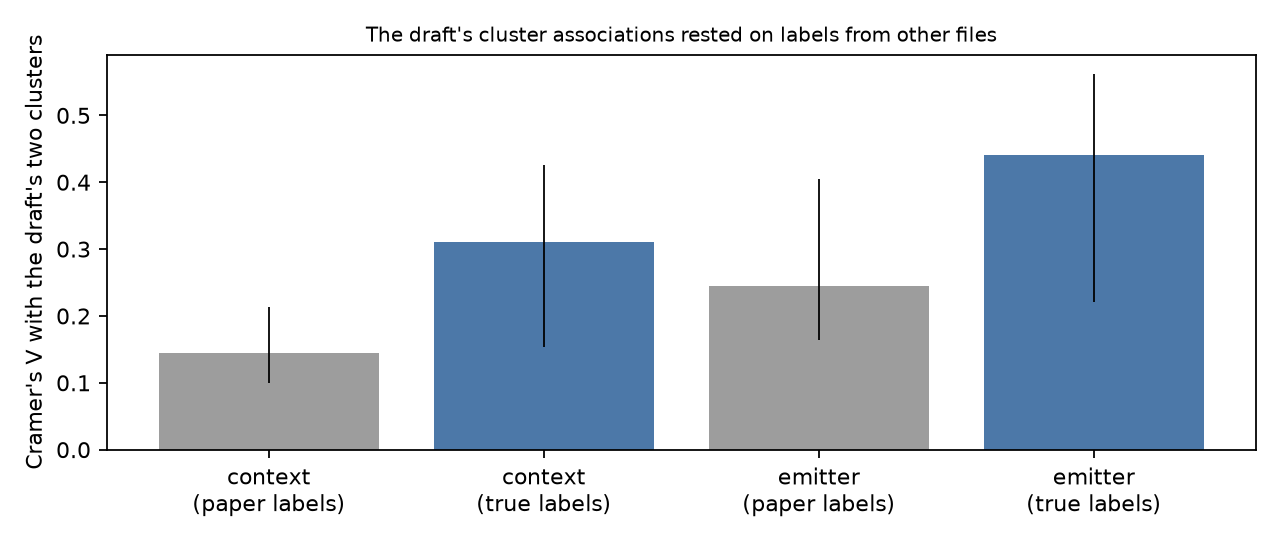
\includegraphics[width=0.62\textwidth]{step3f_draft_true_labels.png}
\caption{\textbf{Figure S1.} Cram\'er's $V$ between the original two clusters and context or emitter, with the labels used in the original manuscript (grey) and with the true labels of the clustered audio (blue). Error bars: 95\% CI resampling whole bats.}
\end{figure}
\begin{figure}[htbp]\centering
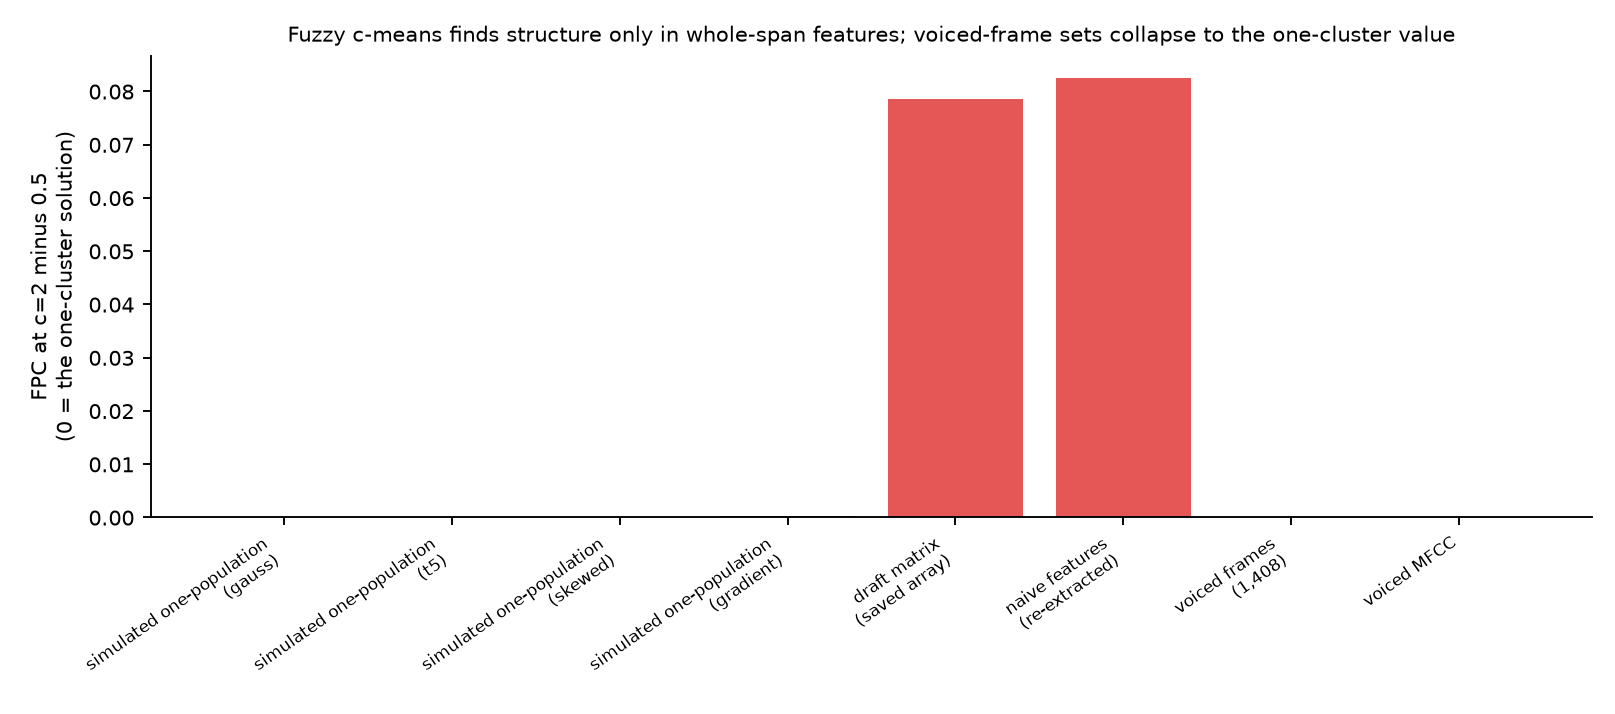
\includegraphics[width=0.85\textwidth]{fig2_fpc_excess_over_one_cluster.png}
\caption{\textbf{Figure S2.} Fuzzy partition coefficient (FPC) at $c=2$ minus 0.5 for simulated one-population data (Gaussian, $t_5$, skewed, curved gradient), the original matrix and the re-extracted feature sets. Voiced-frame sets equal the one-cluster value (0).}
\end{figure}

\paragraph{What HDBSCAN returns.} On 41,116 files, HDBSCAN at minimum size 25 returned one cluster holding 90--92\% of files plus a micro-cluster of 141--152 files (0.3--0.4\%) for the whole-span and voiced features, with 7--10\% of points labelled noise (the noise points had short voiced durations, median 0.09\,s against 0.20\,s); in voiced-MFCC space it returned one cluster of 25\% of files with long voiced durations (median 0.59\,s against 0.14\,s) and 75\% noise; at minimum size 100 it found only clusters of 0.3--5.8\% of files (again longer voiced durations) with 92--100\% noise. Gaussian-mixture BIC and ICL were lowest at the largest $k$ allowed (6) in every set. Held-out-bat stability of the $k=2$ solutions of $k$-means, mixtures and FCM ranged from 0.46 to 0.85 with wide intervals. On 6,000-point subsamples Ward, spectral and BIRCH clustering also had their highest silhouette at $k=2$ (0.12--0.33, falling monotonically with $k$), and DBSCAN's cluster count changed with its radius (1--4 clusters, 4--36\% noise).

\paragraph{Sensitivity to preprocessing.} Table~S6 repeats the main voiced-feature analyses with 5 to 100 principal components and with other scalings. FCM collapses to its one-cluster solution with at least 20 standardised components (and with rank-normal scores), but not with 5--10 components or without standardisation; in those cases its two-way label follows silence and voiced duration (orientation-free AUC 0.72--0.78 and 0.75--0.81) and isolates the Isolation group poorly (F1 0.21--0.22). Prediction strength stays at 0.71--0.77, below the copula null (0.95), the dip $p$ is 0.99 in every configuration, and the bat-blocked Isolation AUC is 0.976--0.984 in every configuration.
\begin{table}[htbp]\centering\scriptsize
\caption{\textbf{Table S6.} Sensitivity of the voiced-feature conclusions to preprocessing and the number of principal components (PCs), 12,000 files. FPC$-$0.5 = fuzzy partition coefficient excess at $c=2$; $k$-means sil. = silhouette at $k=2$; PS = prediction strength at $k=2$ (halves split by bat); dip $p$ = median split-sample dip $p$ value; Isolation AUC from all 41,116 files with folds blocked by bat; the last two columns give the orientation-free AUC of the fuzzy $c=2$ label against silence fraction and voiced duration.}\label{tab:S6}
\begin{adjustbox}{max width=\linewidth}
\begin{tabular}{llccccccc}
\toprule
preprocessing & PCs & FPC$-$0.5 & $k$-means sil. & PS & dip $p$ (median) & Isolation AUC & label vs silence & label vs duration \\
\midrule
standardise & 5 & 0.090 & 0.225 & 0.720 & 0.991 & 0.976 & 0.71 & 0.75 \\
standardise & 10 & 0.024 & 0.177 & 0.722 & 0.992 & 0.980 & 0.72 & 0.75 \\
standardise & 20 & 0.000 & 0.158 & 0.714 & 0.993 & 0.982 & 0.73 & 0.77 \\
standardise & 50 & 0.000 & 0.141 & 0.717 & 0.994 & 0.983 & 0.73 & 0.76 \\
standardise & 100 & 0.000 & 0.133 & 0.716 & 0.993 & 0.983 & 0.73 & 0.76 \\
no scaling & 50 & 0.112 & 0.253 & 0.767 & 0.995 & 0.977 & 0.78 & 0.81 \\
rank normal scores & 50 & 0.000 & 0.146 & 0.744 & 0.995 & 0.984 & 0.74 & 0.77 \\
\bottomrule
\end{tabular}
\end{adjustbox}
\end{table}


\section{Power of the one-cluster-allowed battery}
\paragraph{Design and detection rule.} Two-type mixtures were spiked into the session-mean null (templates of 6,000 rows; minority share 5, 20 and 50\%; separation 1--8 SD along a random direction in the top ten principal components; spikes independent of bat). Every cell was simulated \POWERREPS{} times (Tables~S2a, voiced file-level features, and S2b, syllable shapes; Fig.~2 of the main text shows S2a). A statistic detects the structure when it exceeds the 95th percentile of its distribution in \POWERNULL{} independent no-structure null datasets. This threshold is estimated once per data set and statistic from those null datasets, with their own random seeds, and is not recomputed for each cell; the null and spiked datasets pass through the same reduced-setting pipeline (Section~S0). The false-positive rate of each statistic is therefore 5\% by construction, up to the Monte Carlo error of a 95th percentile estimated from \POWERNULL{} nulls. Intervals in the tables are 95\% Wilson score intervals for a binomial proportion with the stated number of replicates.
\paragraph{Results and comparison with the first run.} For two equally common types the four statistics detected the mixture in 90--100\% of replicates at 4 SD (80--92\% for syllable shapes), 48--70\% at 3 SD (30--34\%) and at most 15\% at 2 SD; a 20\% minority needed 6 SD (96--100\%; 83--99\% for syllables); and a 5\% minority was detected at 8 SD only by the dip statistic (90\%; 64\% for syllables) and at most 18\% (9\%) by any of the four statistics at 6 SD or less. The Wilson half-widths are at most 7 percentage points with 200 replicates (up to 22 with the 20 replicates of the first run). The first run (20 replicates per cell, 40 null datasets) is a subset of this one: its 20 replicates per cell were reproduced exactly (maximum difference 0.0), and the rates agree within Monte Carlo error for the voiced file-level features, while for syllable shapes the rates at 4 SD are lower with 200 replicates (80--92\% instead of 90--100\%). The main text and Fig.~2 use the 200-replicate run.
\begin{table}[htbp]\centering\scriptsize
\caption{\textbf{Table S2a.} Detection rate of the one-cluster-allowed battery for a two-type mixture spiked into a null of voiced file-level features, with 95\% Wilson intervals (200 simulated datasets per row). Minority = share of rows shifted; separation = shift in standard deviations (SD) along a random direction in the top ten principal components. Detection = statistic above the 95th percentile of the no-structure null (fixed once per data set from 200 independent null datasets, not re-estimated per row); PS = prediction strength, dip = split-sample Hartigan dip (statistic, or median $p<0.05$), FPC$>0.01$ = fuzzy partition coefficient excess above 0.01.}\label{tab:S2a}
\begin{adjustbox}{max width=\linewidth}
\begin{tabular}{llcccccc}
\toprule
minority & separation (SD) & PS & silhouette & Jaccard & dip stat. & dip $p<.05$ & FPC$>0.01$ \\
\midrule
5\% & 1 & 0.06 [0.03, 0.10] & 0.01 [0.00, 0.04] & 0.04 [0.02, 0.08] & 0.03 [0.01, 0.06] & 0.00 [0.00, 0.02] & 0.00 [0.00, 0.02] \\
5\% & 2 & 0.10 [0.06, 0.14] & 0.04 [0.02, 0.07] & 0.02 [0.01, 0.05] & 0.04 [0.02, 0.08] & 0.00 [0.00, 0.02] & 0.00 [0.00, 0.02] \\
5\% & 3 & 0.07 [0.04, 0.11] & 0.07 [0.04, 0.11] & 0.05 [0.03, 0.09] & 0.06 [0.03, 0.10] & 0.00 [0.00, 0.02] & 0.00 [0.00, 0.02] \\
5\% & 4 & 0.06 [0.03, 0.10] & 0.06 [0.03, 0.10] & 0.07 [0.04, 0.11] & 0.02 [0.01, 0.05] & 0.00 [0.00, 0.02] & 0.00 [0.00, 0.02] \\
5\% & 6 & 0.07 [0.04, 0.11] & 0.12 [0.08, 0.17] & 0.05 [0.03, 0.09] & 0.18 [0.13, 0.24] & 0.00 [0.00, 0.02] & 0.00 [0.00, 0.02] \\
5\% & 8 & 0.33 [0.26, 0.39] & 0.17 [0.13, 0.23] & 0.27 [0.21, 0.33] & 0.90 [0.84, 0.93] & 0.48 [0.41, 0.55] & 0.00 [0.00, 0.02] \\
20\% & 1 & 0.07 [0.04, 0.11] & 0.03 [0.01, 0.06] & 0.04 [0.02, 0.08] & 0.07 [0.04, 0.11] & 0.00 [0.00, 0.02] & 0.00 [0.00, 0.02] \\
20\% & 2 & 0.11 [0.07, 0.16] & 0.12 [0.09, 0.18] & 0.07 [0.05, 0.12] & 0.05 [0.03, 0.09] & 0.00 [0.00, 0.02] & 0.00 [0.00, 0.02] \\
20\% & 3 & 0.14 [0.10, 0.19] & 0.26 [0.20, 0.32] & 0.17 [0.12, 0.23] & 0.04 [0.02, 0.08] & 0.00 [0.00, 0.02] & 0.01 [0.01, 0.04] \\
20\% & 4 & 0.52 [0.45, 0.59] & 0.50 [0.43, 0.57] & 0.47 [0.40, 0.54] & 0.64 [0.57, 0.70] & 0.20 [0.15, 0.26] & 0.10 [0.06, 0.14] \\
20\% & 6 & 1.00 [0.98, 1.00] & 0.96 [0.92, 0.98] & 0.99 [0.96, 1.00] & 1.00 [0.98, 1.00] & 1.00 [0.98, 1.00] & 0.60 [0.54, 0.67] \\
20\% & 8 & 1.00 [0.98, 1.00] & 0.99 [0.97, 1.00] & 1.00 [0.98, 1.00] & 1.00 [0.98, 1.00] & 1.00 [0.98, 1.00] & 0.95 [0.92, 0.98] \\
50\% & 1 & 0.06 [0.03, 0.10] & 0.04 [0.02, 0.07] & 0.06 [0.03, 0.10] & 0.01 [0.01, 0.04] & 0.00 [0.00, 0.02] & 0.00 [0.00, 0.02] \\
50\% & 2 & 0.12 [0.09, 0.18] & 0.15 [0.11, 0.21] & 0.10 [0.07, 0.16] & 0.04 [0.02, 0.08] & 0.00 [0.00, 0.02] & 0.01 [0.00, 0.03] \\
50\% & 3 & 0.51 [0.44, 0.57] & 0.56 [0.49, 0.62] & 0.47 [0.41, 0.54] & 0.69 [0.63, 0.75] & 0.34 [0.28, 0.41] & 0.16 [0.12, 0.22] \\
50\% & 4 & 0.95 [0.92, 0.98] & 0.90 [0.85, 0.93] & 0.95 [0.92, 0.98] & 0.99 [0.97, 1.00] & 0.97 [0.94, 0.99] & 0.68 [0.61, 0.74] \\
50\% & 6 & 1.00 [0.98, 1.00] & 1.00 [0.98, 1.00] & 1.00 [0.98, 1.00] & 1.00 [0.98, 1.00] & 1.00 [0.98, 1.00] & 0.99 [0.97, 1.00] \\
50\% & 8 & 1.00 [0.98, 1.00] & 1.00 [0.98, 1.00] & 1.00 [0.98, 1.00] & 1.00 [0.98, 1.00] & 1.00 [0.98, 1.00] & 1.00 [0.98, 1.00] \\
\bottomrule
\end{tabular}
\end{adjustbox}
\end{table}

\begin{table}[htbp]\centering\scriptsize
\caption{\textbf{Table S2b.} Detection rate of the one-cluster-allowed battery for a two-type mixture spiked into a null of syllable shapes, with 95\% Wilson intervals (200 simulated datasets per row). Minority = share of rows shifted; separation = shift in standard deviations (SD) along a random direction in the top ten principal components. Detection = statistic above the 95th percentile of the no-structure null (fixed once per data set from 200 independent null datasets, not re-estimated per row); PS = prediction strength, dip = split-sample Hartigan dip (statistic, or median $p<0.05$), FPC$>0.01$ = fuzzy partition coefficient excess above 0.01.}\label{tab:S2b}
\begin{adjustbox}{max width=\linewidth}
\begin{tabular}{llcccccc}
\toprule
minority & separation (SD) & PS & silhouette & Jaccard & dip stat. & dip $p<.05$ & FPC$>0.01$ \\
\midrule
5\% & 1 & 0.01 [0.01, 0.04] & 0.03 [0.01, 0.06] & 0.03 [0.01, 0.06] & 0.03 [0.01, 0.06] & 0.00 [0.00, 0.02] & 0.00 [0.00, 0.02] \\
5\% & 2 & 0.05 [0.03, 0.09] & 0.03 [0.01, 0.06] & 0.03 [0.01, 0.06] & 0.03 [0.01, 0.06] & 0.00 [0.00, 0.02] & 0.00 [0.00, 0.02] \\
5\% & 3 & 0.03 [0.01, 0.06] & 0.04 [0.02, 0.08] & 0.02 [0.01, 0.05] & 0.07 [0.04, 0.11] & 0.00 [0.00, 0.02] & 0.00 [0.00, 0.02] \\
5\% & 4 & 0.04 [0.02, 0.08] & 0.04 [0.02, 0.08] & 0.03 [0.01, 0.06] & 0.03 [0.01, 0.06] & 0.00 [0.00, 0.02] & 0.00 [0.00, 0.02] \\
5\% & 6 & 0.07 [0.04, 0.11] & 0.07 [0.05, 0.12] & 0.04 [0.02, 0.08] & 0.09 [0.05, 0.13] & 0.00 [0.00, 0.02] & 0.00 [0.00, 0.02] \\
5\% & 8 & 0.17 [0.12, 0.23] & 0.12 [0.08, 0.17] & 0.14 [0.09, 0.19] & 0.64 [0.57, 0.70] & 0.30 [0.24, 0.37] & 0.01 [0.00, 0.03] \\
20\% & 1 & 0.03 [0.01, 0.06] & 0.02 [0.01, 0.05] & 0.04 [0.02, 0.07] & 0.03 [0.01, 0.06] & 0.00 [0.00, 0.02] & 0.00 [0.00, 0.02] \\
20\% & 2 & 0.04 [0.02, 0.08] & 0.08 [0.05, 0.13] & 0.03 [0.01, 0.06] & 0.04 [0.02, 0.08] & 0.00 [0.00, 0.02] & 0.00 [0.00, 0.02] \\
20\% & 3 & 0.09 [0.06, 0.14] & 0.20 [0.15, 0.26] & 0.08 [0.05, 0.13] & 0.03 [0.01, 0.06] & 0.00 [0.00, 0.02] & 0.04 [0.02, 0.07] \\
20\% & 4 & 0.27 [0.21, 0.33] & 0.38 [0.32, 0.45] & 0.28 [0.22, 0.34] & 0.38 [0.32, 0.45] & 0.07 [0.04, 0.11] & 0.11 [0.07, 0.16] \\
20\% & 6 & 0.95 [0.92, 0.98] & 0.83 [0.77, 0.88] & 0.94 [0.89, 0.96] & 0.99 [0.96, 1.00] & 0.98 [0.95, 0.99] & 0.52 [0.45, 0.58] \\
20\% & 8 & 1.00 [0.98, 1.00] & 0.98 [0.96, 0.99] & 1.00 [0.98, 1.00] & 1.00 [0.98, 1.00] & 1.00 [0.98, 1.00] & 0.89 [0.84, 0.93] \\
50\% & 1 & 0.04 [0.02, 0.07] & 0.04 [0.02, 0.07] & 0.05 [0.03, 0.09] & 0.05 [0.03, 0.09] & 0.00 [0.00, 0.02] & 0.00 [0.00, 0.02] \\
50\% & 2 & 0.07 [0.05, 0.12] & 0.12 [0.08, 0.17] & 0.07 [0.04, 0.11] & 0.01 [0.01, 0.04] & 0.00 [0.00, 0.02] & 0.02 [0.01, 0.05] \\
50\% & 3 & 0.32 [0.26, 0.39] & 0.34 [0.28, 0.41] & 0.29 [0.24, 0.36] & 0.34 [0.28, 0.41] & 0.11 [0.07, 0.16] & 0.18 [0.14, 0.24] \\
50\% & 4 & 0.83 [0.77, 0.88] & 0.81 [0.75, 0.86] & 0.80 [0.74, 0.85] & 0.92 [0.87, 0.95] & 0.86 [0.81, 0.90] & 0.59 [0.53, 0.66] \\
50\% & 6 & 1.00 [0.98, 1.00] & 1.00 [0.98, 1.00] & 1.00 [0.98, 1.00] & 1.00 [0.98, 1.00] & 1.00 [0.98, 1.00] & 0.99 [0.97, 1.00] \\
50\% & 8 & 1.00 [0.98, 1.00] & 1.00 [0.98, 1.00] & 1.00 [0.98, 1.00] & 1.00 [0.98, 1.00] & 1.00 [0.98, 1.00] & 1.00 [0.98, 1.00] \\
\bottomrule
\end{tabular}
\end{adjustbox}
\end{table}

\begin{figure}[htbp]\centering
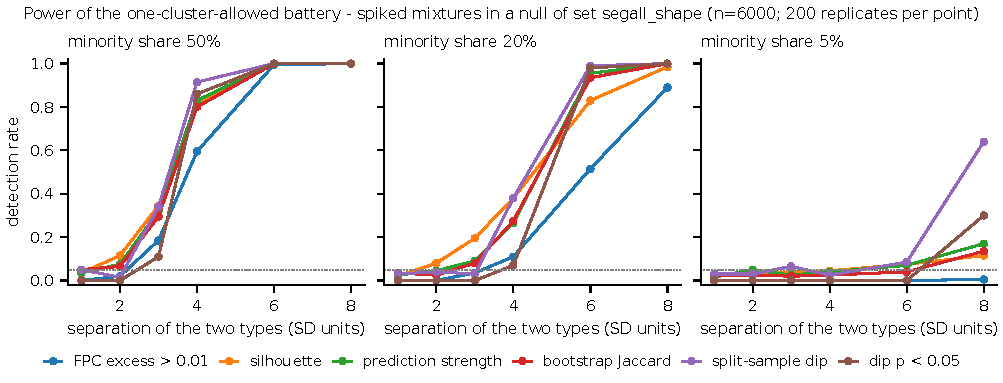
\includegraphics{fig_s5_v4.pdf}
\caption{\textbf{Figure S5.} Detection rate of the one-cluster-allowed battery for two-type mixtures spiked into a null of syllable shapes (6,000 syllables, \POWERREPS{} replicates per point). Panels: minority share of 50\%, 20\% and 5\%; x-axis: separation of the two types in SD; y-axis: detection rate; dotted line: 5\%. FPC, fuzzy partition coefficient; dip, split-sample Hartigan dip.}
\end{figure}
\paragraph{Not tested.} Each replicate used one random direction and spikes independent of bat. Robustness to other directions, to effect structures that are not a mean shift, and to dependence among the recordings of one bat was not simulated; the power estimates therefore apply to this idealised alternative and the main text states only that well-separated common types would have been detected.

\section{Syllable-level analyses}
\paragraph{Duration.} Tables~S9a and S9b give the sample sizes, the Hartigan dip statistic with bat-level bootstrap intervals, and the one- versus two-Gaussian comparison for log$_{10}$ duration; Fig.~S3 shows the distribution. Duration alone carried no context information on unseen bats (balanced accuracy 0.066; 13 contexts, chance 0.077), whereas duration-free spectro-temporal shape did (0.198; accuracy 0.508 against a 0.344 majority rate). For shape, HDBSCAN found two clusters at the smaller minimum size with half of the points labelled noise; for the seven scalar descriptors (duration, SNR and spectral measures) FCM had FPC 0.609 and silhouette 0.262.
\begin{figure}[htbp]\centering
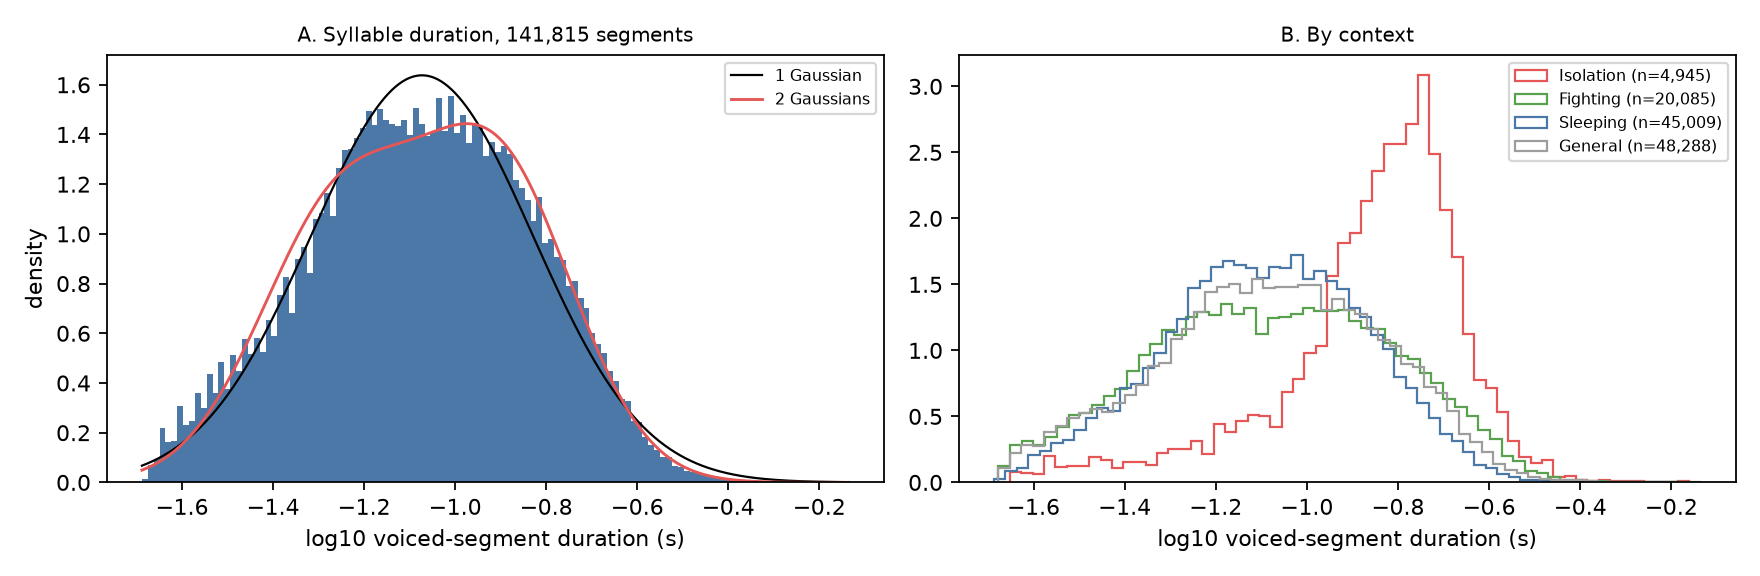
\includegraphics[width=\textwidth]{fig5_segment_duration.png}
\caption{\textbf{Figure S3.} (A) Distribution of $\log_{10}$ syllable duration with one- and two-Gaussian fits (141,815 syllables, 42 bat groups). (B) By context. No bimodality is detectable (Tables S9a, S9b).}
\end{figure}
\begin{table}[htbp]\centering\scriptsize
\caption{\textbf{Table S9a.} Modality of log$_{10}$ syllable duration: number of syllables and bat groups, Hartigan dip statistic with a 95\% interval from 100 bootstrap resamples of whole bats, the dip $p$ value (syllables treated as independent, so optimistic), and median (5th--95th percentile) duration in ms. All syllables of the 30,000-syllable analysis set that have a context label of at least 500 syllables are listed per context.}\label{tab:S9a}
\begin{adjustbox}{max width=\linewidth}
\begin{tabular}{lrrccc}
\toprule
subset & syllables & bats & dip [95\% CI] & dip $p$ & duration, ms \\
\midrule
all segments & 141,815 & 42 & 0.0012 [0.0010, 0.0016] & 0.18 & 85 (32--207) \\
context = Isolation & 4,945 & 24 & 0.0053 [0.0047, 0.0144] & 0.52 & 151 (51--249) \\
context = Fighting & 20,085 & 41 & 0.0032 [0.0022, 0.0061] & 0.19 & 85 (31--222) \\
context = Sleeping & 45,009 & 42 & 0.0021 [0.0014, 0.0029] & 0.26 & 82 (34--182) \\
context = General & 48,288 & 42 & 0.0014 [0.0013, 0.0022] & 0.81 & 84 (31--202) \\
context = Feeding & 7,639 & 40 & 0.0047 [0.0036, 0.0075] & 0.33 & 85 (33--191) \\
context = Mating protest & 7,094 & 30 & 0.0030 [0.0032, 0.0107] & 0.98 & 77 (31--266) \\
\bottomrule
\end{tabular}
\end{adjustbox}
\end{table}

\begin{table}[htbp]\centering\scriptsize
\caption{\textbf{Table S9b.} One- versus two-component Gaussian mixtures for log$_{10}$ syllable duration (141,815 syllables, 42 bat groups): Bayesian information criterion (BIC; lower is better; 3 initialisations, seed 42) and its difference to the best number of components. A positive BIC(1) $-$ BIC(2) favours two components; the interval resamples whole bats. Two-component fit: means [56.0, 124.6] ms, weights [0.485, 0.515]. A lower BIC for more components is expected for a smooth, skewed distribution and is not evidence of discrete duration classes (dip test in Table S9a).}\label{tab:S9b}
\begin{adjustbox}{max width=\linewidth}
\begin{tabular}{lcc}
\toprule
components & BIC & $\Delta$BIC vs best \\
\midrule
1 & 1,851 & 2,825 \\
2 & -226 & 749 \\
3 & -505 & 469 \\
4 & -939 & 35 \\
5 & -887 & 87 \\
6 & -974 & 0 \\
BIC(1) $-$ BIC(2) [95\% CI] & 2,077 [764, 4,237] & 200 bat-level resamples \\
\bottomrule
\end{tabular}
\end{adjustbox}
\end{table}


\section{Learned and pretrained representations}
Table~S8 summarises the comparison of the handcrafted syllable shape with the VAE latent space (trained on 21 bats, tested on the 21 others) and the AVES embeddings. None of the learned or pretrained representations revealed discrete structure or more context information than handcrafted features. Extraction of AVES embeddings cost 4.4--9.9\,s per file on a CPU (depending on load).

\begin{table}[htbp]\centering\tiny
\caption{\textbf{Table S8.} Handcrafted, learned and pretrained representations compared. Null values are means of the Gaussian-copula and session-mean nulls (cop./ses.). PS, prediction strength; Jaccard, bootstrap Jaccard stability; sil., silhouette; FPC, fuzzy partition coefficient; bal.\ acc., balanced accuracy of leave-bats-out decoding of context (chance in brackets).}
\begin{adjustbox}{max width=\linewidth}
\begin{tabular}{p{2.0cm}p{2.0cm}p{5.8cm}p{3.7cm}p{3.3cm}}
\toprule
representation & held-out unit & clusterability evidence (observed vs null) & context information & limitation \\
\midrule
Handcrafted syllable shape (512 values; 30,000 syllables, 36 bats) & bats (PS, Jaccard, dip; decoding folds) & FCM FPC 0.500; PS 0.73 \ci{0.68}{0.87} vs 0.97/0.83; Jaccard 0.94 vs 0.99/0.95; silhouette 0.152 vs 0.141/0.144; dip 0.0017 vs 0.0018/0.0017, median $p=0.995$ & bal.\ acc.\ 0.198 (0.077); duration alone 0.066 & syllables of one segmentation; 13 contexts \\
VAE latent (8-D; KL weight 0.1 and 1) & 21 unseen bats (13,510 syllables) & FCM FPC 0.500; PS 0.67 vs 0.89/0.64; Jaccard 0.85 vs 0.95/0.86; silhouette 0.091 vs 0.104 (copula); dip 0.0028 vs 0.0026, $p=0.22$; $k$-means silhouette at $k=2$ 0.14 and 0.11; reconstruction $R^2$ 0.658 and 0.660 & bal.\ acc.\ 0.157--0.165 (12 contexts) & one small architecture; trained on 21 bats \\
8-PC linear baseline (same syllables) & 21 unseen bats & PS 0.51 vs 0.86/0.53; Jaccard 0.73 vs 0.93/0.76; silhouette 0.082 vs 0.090; dip 0.0028 vs 0.0026; $k$-means silhouette 0.115; reconstruction $R^2$ 0.620; held-out-bat stability of the $k=2$ solutions 0.02--0.30 (intervals reaching zero) for the baseline and VAE variants, except 0.53 \ci{0.21}{0.72} for $k$-means in the better latent space & bal.\ acc.\ 0.167 & linear reference only \\
AVES (2 models $\times$ 4 variants) & 1,000 files; decoding folds blocked by bat & FCM FPC 0.500 in 8 of 8 variants (handcrafted whole-span 0.570); $k$-means silhouette 0.14--0.18 in 7 of 8, the exception (plain whole-span \texttt{aves-base-all}, 0.41) split files by recording channel (NMI 0.165 vs 0.026 with context); HDBSCAN found structure in 2 of 16 settings (62\% and 11\% noise) & bal.\ acc.\ 0.19--0.27 (0.077); handcrafted 0.24--0.25; Isolation AUC 0.93--0.95 vs 0.94--0.97 (114 Isolation files, 14 bats) & only 1,000 files; voiced AVES carried the least channel information (0.19--0.22 vs 0.32--0.51) \\
\bottomrule
\end{tabular}
\end{adjustbox}
\end{table}

\section{The Isolation group: further analyses}
\paragraph{Separability under controls.} Table~S4 gives the AUC of the leave-bats-out Isolation score under the controls described in the main text. Table~S4b gives the sample sizes (recordings, Isolation and other-context recordings, unique bats) and bat-level bootstrap intervals for each age window and for each held-out channel and treatment. Isolation recordings span 10 of 12 channels (channels 1, 2, 3, 4, 9, 11 and 12 each hold at least 93 Isolation files from 4--13 bats) and 24 bats, 57\% of them with the unknown-emitter code; three channels hold almost none (5, 7, 8).
\begin{table}[htbp]\centering\scriptsize
\caption{\textbf{Table S4.} Separability of pups' Isolation calls from all other contexts, as the area under the ROC curve (AUC; 0.5 = none) of out-of-fold scores of a balanced logistic regression on 50 principal components, for voiced file-level features (41,116 files) and syllable shapes (30,000 syllables). Validation unit: whole bats (five folds blocked by bat) unless the row states another held-out unit; brackets are 95\% intervals from resampling whole bats; ranges and counts refer to the groups listed in the row (Table S4b gives each group's sample size).}\label{tab:S4}
\begin{adjustbox}{max width=\linewidth}
\begin{tabular}{lcc}
\toprule
analysis & voiced file features & syllable shape \\
\midrule
all files, folds blocked by bat & 0.984 [0.979, 0.991] & 0.956 [0.944, 0.974] \\
pups only, folds blocked by bat & 0.982 [0.969, 0.990] & 0.951 [0.920, 0.975] \\
pups only, within channel$\times$month strata (weighted mean) & 0.902 & 0.846 \\
without the unknown-emitter group (57\% of Isolation files) & 0.984 [0.974, 0.992] & 0.952 [0.926, 0.974] \\
per identified pup (median; range; number of pups) & 0.971; 0.83--1.00; 15 & 0.942; 0.71--1.00; 14 \\
each channel held out (weighted mean; range; number) & 0.983; 0.93--0.99; 8 & 0.945; 0.89--0.98; 7 \\
each treatment held out (weighted mean; range; number) & 0.986; 0.95--1.00; 6 & 0.954; 0.92--0.97; 6 \\
pup age windows (file-weighted mean over windows with at least 15 recordings per class; per window in Table S4b) & 0.931 & 0.876 \\
\bottomrule
\end{tabular}
\end{adjustbox}
\end{table}

\begin{table}[htbp]\centering\scriptsize
\caption{\textbf{Table S4b.} Isolation versus other contexts within strata: recordings (files or syllables), Isolation (positive) and other-context (negative) counts, number of unique bats (pups for age windows) and AUC of the leave-bats-out score with a 95\% percentile interval from 1,000 bootstrap resamples of whole bats. Age windows are days since birth for the 20 pups with known birth dates (pup age stratum), evaluated only with at least 15 recordings per class; the windows were fixed once at analysis time as an exploratory control after the Isolation group had been found, not pre-specified. Channel/treatment held out: model trained on all other channels (treatments), scored on the held-out one; evaluated only with at least 20 per class. Intervals reflect resampling of bats among scored recordings and do not include model-fitting variability. Youngest pups (0--40 days) contribute almost only Isolation recordings, so age and context cannot be separated there, and the lower AUC at 40--60 days should not be read as the same distinctness at every developmental stage.}\label{tab:S4b}
\begin{adjustbox}{max width=\linewidth}
\begin{tabular}{llrrrrrl}
\toprule
stratum & features & group & recordings & Isolation & other & bats & AUC [95\% CI] \\
\midrule
pup age (days) & voiced file features & [0, 20) & 74 & 74 & 0 & 9 & not evaluated (< 15 per class) \\
 & voiced file features & [20, 40) & 113 & 109 & 4 & 16 & not evaluated (< 15 per class) \\
 & voiced file features & [40, 60) & 485 & 352 & 133 & 18 & 0.698 [0.613, 0.781] \\
 & voiced file features & [60, 90) & 1,275 & 584 & 691 & 20 & 0.929 [0.890, 0.957] \\
 & voiced file features & [90, 150) & 2,749 & 44 & 2,705 & 16 & 0.973 [0.918, 0.996] \\
 & voiced file features & [150, 400) & 6,491 & 13 & 6,478 & 16 & not evaluated (< 15 per class) \\
 & syllable shape & [0, 20) & 36 & 36 & 0 & 9 & not evaluated (< 15 per class) \\
 & syllable shape & [20, 40) & 55 & 52 & 3 & 13 & not evaluated (< 15 per class) \\
 & syllable shape & [40, 60) & 196 & 138 & 58 & 18 & 0.720 [0.601, 0.823] \\
 & syllable shape & [60, 90) & 659 & 225 & 434 & 20 & 0.906 [0.851, 0.940] \\
 & syllable shape & [90, 150) & 1,531 & 20 & 1,511 & 16 & 0.883 [0.629, 0.980] \\
 & syllable shape & [150, 400) & 3,935 & 3 & 3,932 & 16 & not evaluated (< 15 per class) \\
channel held out & voiced file features & 1 & 14,854 & 952 & 13,902 & 20 & 0.988 [0.971, 0.994] \\
 & voiced file features & 2 & 3,127 & 279 & 2,848 & 21 & 0.978 [0.950, 0.996] \\
 & voiced file features & 3 & 3,476 & 308 & 3,168 & 11 & 0.980 [0.954, 0.995] \\
 & voiced file features & 4 & 3,353 & 274 & 3,079 & 18 & 0.973 [0.935, 0.996] \\
 & voiced file features & 9 & 818 & 93 & 725 & 14 & 0.981 [0.961, 0.999] \\
 & voiced file features & 10 & 116 & 28 & 88 & 3 & 0.930 [interval not meaningful, 3 bat(s)] \\
 & voiced file features & 11 & 1,790 & 441 & 1,349 & 10 & 0.983 [0.965, 0.997] \\
 & voiced file features & 12 & 3,462 & 304 & 3,158 & 9 & 0.981 [0.941, 0.992] \\
treatment held out & voiced file features & 1 & 2,388 & 481 & 1,907 & 9 & 0.980 [0.959, 0.997] \\
 & voiced file features & 2 & 3,993 & 341 & 3,652 & 8 & 0.979 [0.929, 0.991] \\
 & voiced file features & 9 & 6,133 & 491 & 5,642 & 10 & 0.981 [0.965, 0.995] \\
 & voiced file features & 10 & 5,151 & 1,029 & 4,122 & 13 & 0.980 [0.955, 0.988] \\
 & voiced file features & 13 & 92 & 50 & 42 & 1 & 0.951 [interval not meaningful, 1 bat(s)] \\
 & voiced file features & 17 & 9,930 & 202 & 9,728 & 6 & 0.996 [0.986, 0.999] \\
\bottomrule
\end{tabular}
\end{adjustbox}
\end{table}

\paragraph{Age.} The AUC is clearly lower in the 40--60-day window (0.70, 352 Isolation against 133 other recordings from 18 pups) than at 60--90 days (0.93) and 90--150 days (0.97); the windows were fixed once at analysis time, after the Isolation group had been found, and the interval for the 90--150-day window is wide because it holds 44 Isolation recordings. Pups younger than 40 days contribute almost only Isolation recordings (183 against 4), so age, recording situation and call type cannot be separated in these observational data, and the groups should not be interpreted as equally distinct at every developmental stage. With so few other-context recordings in the youngest windows an age-by-context model would be poorly powered and was not fitted.
\paragraph{Earlier forced two-way split.} In voiced MFCC space a forced two-way $k$-means split produced a small cluster (16.5\% of files) containing 93.3\% of Isolation-context files (2,557/2,740) and 5--24\% of most other contexts (Separation 44\%, Unknown 33\%); it was not explained by SNR (AUC 0.50) or duration (0.46), survived channel$\times$month permutation (NMI 0.311 against a null of 0.021), and contained 95.6\% of pups' Isolation calls, 16.7\% of pups' calls in other contexts and 4.2\% of adults' (Fig.~S4). It was less pure than the UMAP--HDBSCAN cluster (2\% of pups' other calls), and a $k$-means split of syllable shapes put 95.2\% of Isolation syllables in a half that held 49\% of all syllables: such splits of all the data say little about whether Isolation calls form their own mode.
\begin{figure}[htbp]\centering
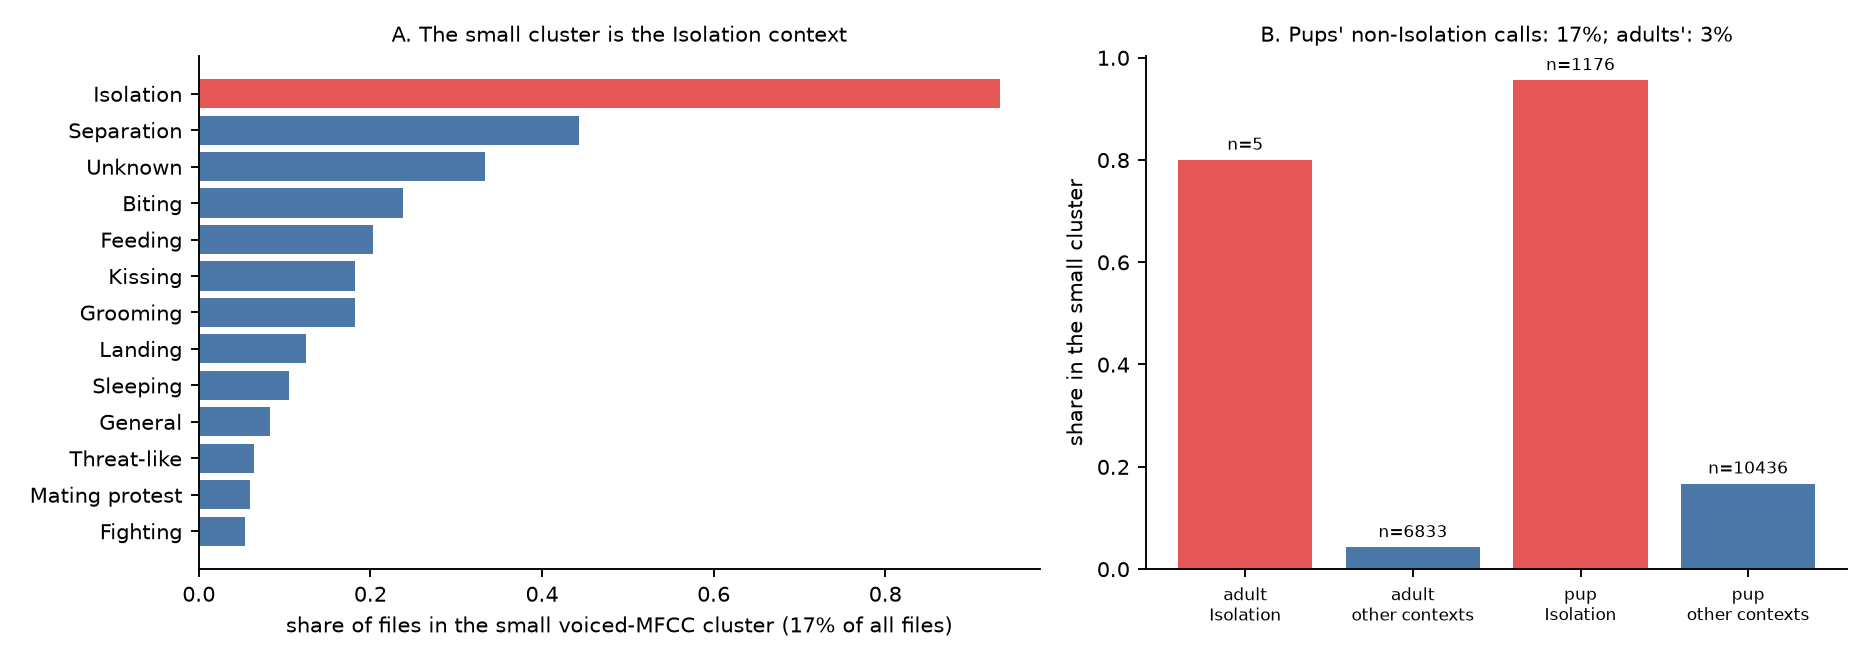
\includegraphics[width=0.9\textwidth]{fig4_isolation_cluster.png}
\caption{\textbf{Figure S4.} (A) Share of files in the small voiced-MFCC $k$-means cluster, by context. (B) Pups versus adults, Isolation versus other contexts (positive-coded bats; $n$ = number of files).}
\end{figure}

\section{Out-of-sample sets}
\paragraph{Sequence of discovery, model choice and evaluation.} Table~S5b and Fig.~S6a give the exact partition. Discovery sample (41,116 files): everything exploratory took place here, namely the development set analysed first (15,992 files, 7--8 October 2026), the discovery of the small cluster by UMAP--HDBSCAN on 12,000 voiced files, the 50-component representation, the logistic-regression settings ($C=0.5$, balanced classes) and the UMAP/HDBSCAN settings (kept at their values at first use and not varied afterwards), and the supervised and stratified tests. The criteria C1--C3 and their thresholds (AUC $\ge0.90$; a cluster of 3--12\% of files with at least 70\% Isolation-context; null datasets fragmenting more than the real data) were written to the chronological analysis log on 8 October 2026 at 09:48 (replication sample) and 15:15 (completion sample), before any file of the respective sample was analysed; the outcome was to be reported whichever way it came out. For the held-out files the standardiser, principal-component transform and Isolation model were fitted on discovery files only; the UMAP and HDBSCAN fits of C2 used the new files alone and no labels (labels were used only to score the purity of the resulting cluster). No feature, model or threshold was selected or tuned on the held-out files, and no setting was changed after seeing their results. After the criteria were fixed, further exploratory analyses (age windows, channel-held-out tests, AVES, harder UMAP nulls) were still run on the discovery sample only.
\paragraph{Same-corpus evaluation.} The replication and completion samples come from the same corpus, colony and recording period as the discovery sample, share all of their positive-coded bats and channels with it, and almost all recording days (Table~S5b). They test whether the finding is an over-fit to the discovery recordings; they are not an independent-colony replication and do not test generalisation to new individuals or recording set-ups, which is addressed only within the discovery sample by bat-, channel-, treatment- and session-blocked evaluation.
\begin{table}[htbp]\centering\scriptsize
\caption{\textbf{Table S5.} Out-of-sample evaluation of the Isolation finding with the pre-specified criteria. C1: AUC of the model trained on discovery files only (95\% interval resampling whole bats, 300 resamples), $d'$ = standardised separation of the Isolation and other-context scores, pups-only AUC; C2: share of files and share of Isolation-context files in the small UMAP--HDBSCAN cluster (fitted on the new files alone); C3: number of clusters and share of points labelled noise, real data versus the mean of six Gaussian-copula null datasets. Samples are described in Table S5b; they share bats and channels with the discovery sample.}\label{tab:S5}
\begin{adjustbox}{max width=\linewidth}
\begin{tabular}{lccccc}
\toprule
sample & C1 AUC [95\% CI] & $d'$ & pups only AUC & C2 share / purity & C3 clusters; noise \\
\midrule
replication sample (12,000) & 0.988 [0.978, 0.992] & 5.09 & 0.985 & 0.058 / 0.901 & 2 vs 8.0; 0.00 vs 0.70 \\
completion sample (33,557) & 0.991 [0.983, 0.995] & 5.11 & 0.989 & 0.056 / 0.915 & 2 vs 7.7; 0.00 vs 0.70 \\
\bottomrule
\end{tabular}
\end{adjustbox}
\end{table}

\begin{table}[htbp]\centering\scriptsize
\caption{\textbf{Table S5b.} Data partitions and sample accounting. Partitions are disjoint sets of annotated files (one annotation row per file); the unit separating them is the recording (file). Bats, channels and recording days overlap: all 33 positive-coded bats of the replication sample and of the completion sample, and all 12 channels, also occur in the discovery sample (recording days: 329 of 330 and 338 of 338 shared), so the out-of-sample sets test over-fitting to the discovery recordings, not generalisation to new individuals, recording set-ups or colonies.}\label{tab:S5b}
\begin{adjustbox}{max width=\linewidth}
\begin{tabular}{lrrrrrrp{5.2cm}}
\toprule
partition & files & Isolation files & positive-coded files & bats & channels & days & role \\
\midrule
discovery & 41,116 & 2,740 & 18,450 & 41 & 12 & 344 & all development, exploratory discovery of the cluster, supervised tests blocked by bat/channel/treatment/age, choice of settings \\
replication & 12,000 & 695 & 4,650 & 33 & 12 & 330 & out-of-sample test of C1--C3 (random draw) \\
completion & 33,557 & 2,089 & 13,344 & 33 & 12 & 338 & second out-of-sample test of C1--C3 (all remaining files) \\
reproduction only & 1,313 & 83 & 1,313 & 10 & 9 & 217 & extracted only to reproduce the June table; not used for any test \\
all annotated files & 87,986 & 5,607 & 37,757 & 41 & 12 & 345 & every annotated file of the corpus (205,252 further recordings are unannotated and unused) \\
\bottomrule
\end{tabular}
\end{adjustbox}
\end{table}

\begin{figure}[htbp]\centering
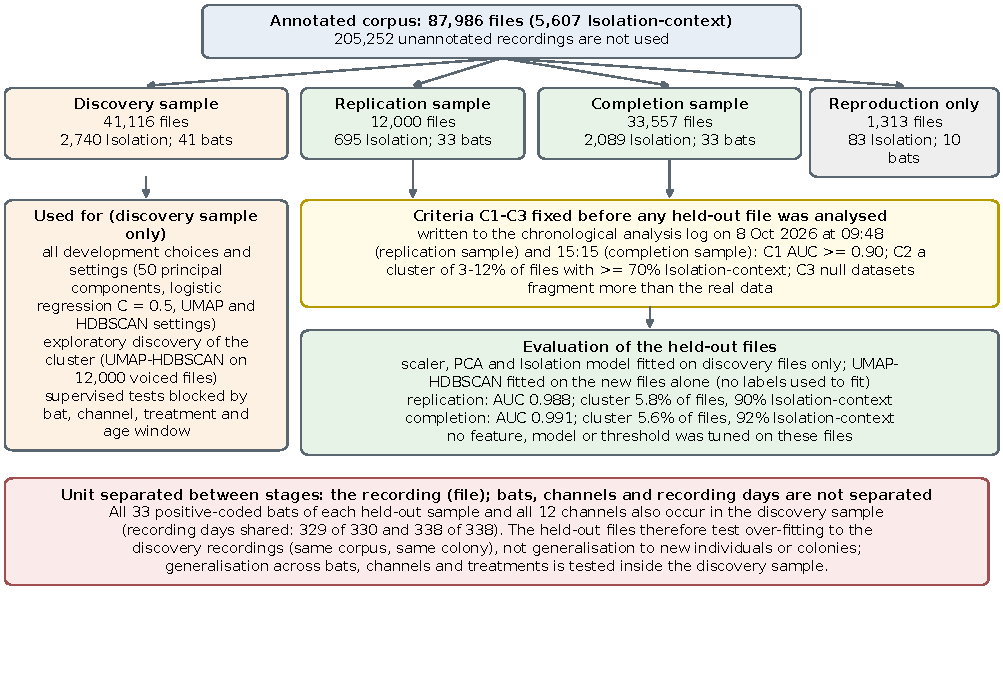
\includegraphics{fig_flow_v4.pdf}
\caption{\textbf{Figure S6a.} Data partitions and the sequence of the Isolation-group analysis: sample sizes from the annotated corpus, the stages at which each partition was used, when the criteria C1--C3 were fixed, and the overlap of bats, channels and recording days between discovery and held-out files.}
\end{figure}
\begin{figure}[!t]\centering
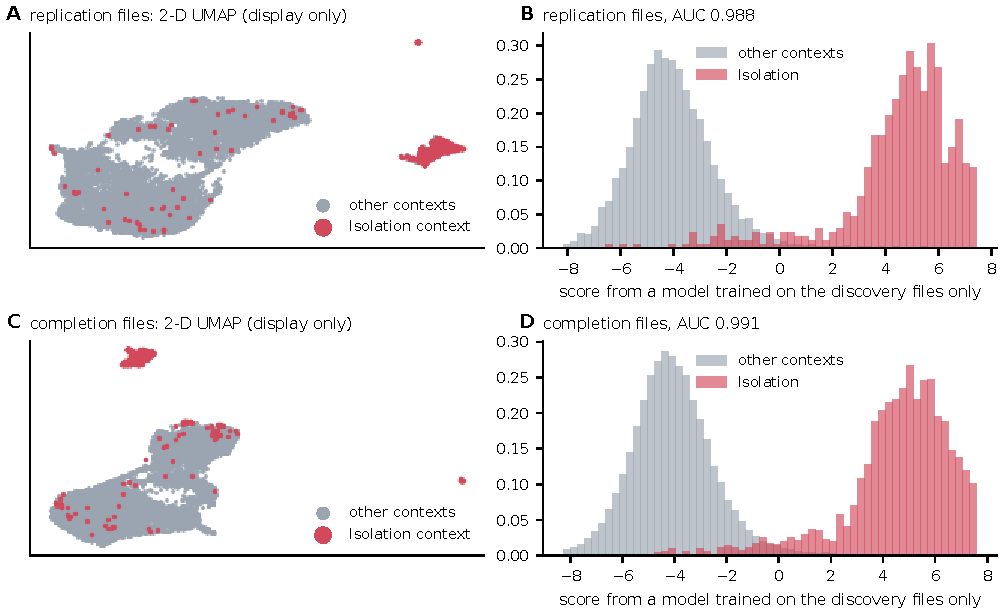
\includegraphics{fig5_v4.pdf}
\caption{\textbf{Figure S6b.} Out-of-sample replication. Top row: 12,000 annotated files never used before. Bottom row: all remaining 33,557 annotated files (UMAP on a seeded 12,000-file subsample). In each row, the left panel is a 2-D UMAP of the new files (display only) with Isolation-context files highlighted and the right panel the score of a model trained on the discovery files only, Isolation versus other contexts (AUC in the panel title; density histograms).}
\end{figure}
\paragraph{Further numbers.} In the completion sample the small UMAP cluster held 82\% of the Isolation files of the 12,000-file subsample, and at minimum size 30 a third micro-cluster of 54 files (96\% Isolation, four emitter groups) appeared. At minimum size 100 the six copula nulls of the replication sample returned 7--10 clusters with 69--72\% noise and those of the completion sample 7--8 clusters with 64--74\% noise (real data: two clusters, at most 0.45\% noise); at minimum size 30, five of the six replication nulls returned two or three clusters with under 1\% noise, so cluster counts alone carry little weight and the supervised result carries the replication. The negative results replicated in both samples: whole-span FCM FPC 0.586 and 0.587 (discovery 0.583) with the two-way label tracking silence fraction (AUC 0.899 and 0.903; discovery 0.887), voiced duration (0.915 and 0.916) and span length (0.842 and 0.842); voiced-feature FPC 0.5000, prediction strength 0.70 and 0.66 against null means 0.95 and 0.955 (null minima 0.93 and 0.945), bootstrap Jaccard stability 0.88 against 0.99, and split-sample dip statistic 0.0027 and 0.0028 against 0.0030 (median dip $p=0.996$ and 0.995).

\section{Identity, channel normalisation and pair-coded calls}
Table~S3 consolidates the emitter-identification results. Accuracy, balanced accuracy and the majority-class baseline are reported separately because accuracy depends on class frequencies and is a poor yardstick when whole channels are held out. The validation unit is stated in the \emph{folds} column; models are fitted on training folds only and bats absent from the training folds are dropped from the test rows.
\begin{table}[htbp]\centering\scriptsize
\caption{\textbf{Table S3.} Emitter identification from file-level features (40 bats) and syllable shapes (36 bats): accuracy with 95\% bat-level bootstrap interval, balanced accuracy, the majority-class accuracy baseline, and, for channel-blocked folds, the mean balanced accuracy over permutations of the labels within channel$\times$month strata (null). Uniform chance (balanced accuracy of a random guess) is 0.025 for 40 bats and 0.028 for 36. 40 bats = the 40 of the 41 positive-coded bats with at least 30 files in the 41,116-file discovery sample (the 41st has 23); 36 = bats with at least 30 of the 30,000 sampled syllables. Rows of bats absent from the training folds are dropped (test rows kept: 100\% except 96\% for channel-blocked). Normalisations use no labels: chan\_mean = per-channel mean subtracted, chan\_z = per-channel standardisation, chanmonth\_mean = per-channel$\times$month mean subtracted; accuracy was not recorded for them (--). Model: multinomial logistic regression on 50 principal components.}\label{tab:S3}
\begin{adjustbox}{max width=\linewidth}
\begin{tabular}{lllcccc}
\toprule
features & normalisation & folds & accuracy [95\% CI] & balanced acc. & majority acc. & null bal. acc. \\
\midrule
voiced 1,408 & none & random 5-fold & 0.593 [0.572, 0.618] & 0.462 & 0.145 & -- \\
voiced 1,408 & none & day-blocked & 0.560 [0.528, 0.588] & 0.423 & 0.145 & -- \\
voiced 1,408 & none & channel-blocked & 0.202 [0.115, 0.255] & 0.125 & 0.152 & 0.036 \\
voiced 1,408 & none & month-blocked & 0.487 [0.399, 0.553] & 0.317 & 0.145 & -- \\
voiced 1,408 & none & archive-blocked & 0.504 [0.455, 0.557] & 0.344 & 0.145 & -- \\
voiced 1,408 & chan\_mean & random 5-fold & -- & 0.437 & -- & -- \\
voiced 1,408 & chan\_mean & day-blocked & -- & 0.396 & -- & -- \\
voiced 1,408 & chan\_mean & channel-blocked & -- & 0.099 & -- & 0.021 \\
voiced 1,408 & chan\_z & random 5-fold & -- & 0.417 & -- & -- \\
voiced 1,408 & chan\_z & day-blocked & -- & 0.377 & -- & -- \\
voiced 1,408 & chan\_z & channel-blocked & -- & 0.088 & -- & 0.017 \\
voiced 1,408 & chanmonth\_mean & random 5-fold & -- & 0.331 & -- & -- \\
voiced 1,408 & chanmonth\_mean & day-blocked & -- & 0.301 & -- & -- \\
voiced 1,408 & chanmonth\_mean & channel-blocked & -- & 0.083 & -- & 0.006 \\
whole-span 1,408 & none & random 5-fold & 0.558 [0.537, 0.580] & 0.441 & 0.145 & -- \\
whole-span 1,408 & none & day-blocked & 0.527 [0.499, 0.553] & 0.399 & 0.145 & -- \\
whole-span 1,408 & none & channel-blocked & 0.220 [0.072, 0.305] & 0.100 & 0.152 & 0.047 \\
whole-span 1,408 & none & month-blocked & 0.448 [0.367, 0.511] & 0.296 & 0.145 & -- \\
whole-span 1,408 & none & archive-blocked & 0.465 [0.417, 0.517] & 0.314 & 0.145 & -- \\
whole-span 1,408 & chan\_mean & random 5-fold & -- & 0.393 & -- & -- \\
whole-span 1,408 & chan\_mean & day-blocked & -- & 0.345 & -- & -- \\
whole-span 1,408 & chan\_mean & channel-blocked & -- & 0.073 & -- & 0.019 \\
whole-span 1,408 & chan\_z & random 5-fold & -- & 0.370 & -- & -- \\
whole-span 1,408 & chan\_z & day-blocked & -- & 0.326 & -- & -- \\
whole-span 1,408 & chan\_z & channel-blocked & -- & 0.064 & -- & 0.020 \\
whole-span 1,408 & chanmonth\_mean & random 5-fold & -- & 0.270 & -- & -- \\
whole-span 1,408 & chanmonth\_mean & day-blocked & -- & 0.243 & -- & -- \\
whole-span 1,408 & chanmonth\_mean & channel-blocked & -- & 0.066 & -- & 0.007 \\
syllable shape (36 bats) & none & random 5-fold & -- & 0.327 & -- & -- \\
syllable shape (36 bats) & none & day-blocked & -- & 0.300 & -- & -- \\
syllable shape (36 bats) & none & channel-blocked & -- & 0.095 & -- & 0.031 \\
syllable shape (36 bats) & chan\_mean & random 5-fold & -- & 0.255 & -- & -- \\
syllable shape (36 bats) & chan\_mean & day-blocked & -- & 0.229 & -- & -- \\
syllable shape (36 bats) & chan\_mean & channel-blocked & -- & 0.056 & -- & 0.011 \\
syllable shape (36 bats) & chan\_z & random 5-fold & -- & 0.246 & -- & -- \\
syllable shape (36 bats) & chan\_z & day-blocked & -- & 0.223 & -- & -- \\
syllable shape (36 bats) & chan\_z & channel-blocked & -- & 0.052 & -- & 0.009 \\
syllable shape (36 bats) & chanmonth\_mean & random 5-fold & -- & 0.196 & -- & -- \\
syllable shape (36 bats) & chanmonth\_mean & day-blocked & -- & 0.182 & -- & -- \\
syllable shape (36 bats) & chanmonth\_mean & channel-blocked & -- & 0.048 & -- & 0.004 \\
\bottomrule
\end{tabular}
\end{adjustbox}
\end{table}

Pooled over 70 bat--channel classes (17,416 files, 970 channel-days) within-channel day-blocked accuracy was 0.648 against a within-channel majority rate of 0.326 ($+0.322$, \ci{0.288}{0.347}). For 16,663 pair-coded files, an identifier trained on positive-coded files assigned a mean probability of 0.461 to the two recognised participants (stratum-shuffle null 0.290; 97.5th percentile 0.293; 0 of 100) and ranked a participant first in 58.7\% of files (null 33.1\%); trained only on other channels, 0.183 against 0.126 and 24.3\% against 14.6\%.

\section{All clustering algorithms}
\paragraph{Selection and admissibility rules.} For each of the 15 algorithms (26 variants) and each of the 19 representations several configurations were run (number of clusters, radius, resolution or minimum size; Section~S0), 1,558 in total. A configuration is \emph{admissible} only if at least two clusters each hold at least 1\% of the points (otherwise single linkage ``wins'' by peeling off singletons). The \emph{best} configuration of a variant on a representation is the admissible one with the highest silhouette of the non-noise points; bat-transfer stability (ARI between a fit on one random half of the bats transferred to the other half and a fit on that half itself, two splits) was computed for the best configuration only, and skipped when a fit took more than 90\,s. Pups' Isolation calls count as \emph{recovered} when one cluster has precision at least 0.7 and recall at least 0.5 for them. Table~S7 summarises the 26 variants; Fig.~S7 shows the best configuration of every algorithm on every representation. All 1,558 configurations are in Supplementary Data SD1 and the best configurations in SD2. On the four file-level representations of Dataset A no variant gave a partition that was at once well separated (silhouette $\ge0.25$), stable across bats (transfer ARI $\ge0.6$) and balanced (larger cluster $\le80\%$ of the files); the main text states the results for the Isolation group.
\begin{table}[htbp]\centering\scriptsize
\caption{\textbf{Table S7.} Fifteen clustering algorithms (26 variants) on 19 representations ($n\le6{,}000$ each): per variant, the number of representations with an admissible partition (at least two clusters holding $\ge1\%$ of the points), the median silhouette of its best configuration, the number of representations whose best configuration has silhouette $\ge0.25$, the median bat-transfer ARI, and the number of the 17 representations with context labels in which the best-silhouette configuration (best) or any configuration (any) contains a cluster with precision $\ge0.7$ and recall $\ge0.5$ for pups' Isolation calls. Silhouette: mean silhouette width of non-noise points (3,000-point subsample); ARI: adjusted Rand index between a half-bat fit transferred to the other half and a fit on that half.}\label{tab:S7}
\begin{adjustbox}{max width=\linewidth}
\begin{tabular}{lcccccc}
\toprule
algorithm / variant & admissible & median sil. & sil.$\ge0.25$ & median transfer ARI & Isolation (best) & Isolation (any) \\
\midrule
k-means & 19 & 0.17 & 4 & 0.58 & 1 & 7 \\
fuzzy c-means & 19 & 0.14 & 2 & 0.53 & 0 & 0 \\
k-medoids (PAM) & 19 & 0.15 & 4 & 0.28 & 1 & 6 \\
ward linkage & 19 & 0.17 & 6 & 0.27 & 5 & 10 \\
average linkage & 7 & 0.28 & 5 & 0.21 & 3 & 3 \\
complete linkage & 17 & 0.26 & 10 & 0.22 & 0 & 1 \\
single linkage & 0 & -- & 0 & -- & 0 & 0 \\
spectral (15-NN) & 19 & 0.25 & 10 & 0.67 & 9 & 13 \\
BIRCH & 19 & 0.17 & 4 & 0.27 & 5 & 10 \\
GMM-spherical & 19 & 0.16 & 3 & 0.47 & 1 & 2 \\
GMM-diag & 19 & 0.13 & 2 & 0.25 & 1 & 5 \\
GMM-tied & 19 & 0.18 & 5 & 0.27 & 6 & 11 \\
GMM-full & 19 & 0.15 & 0 & 0.45 & 2 & 7 \\
Bayesian GMM (Dirichlet process) & 11 & -0.01 & 0 & 0.26 & 0 & 0 \\
DBSCAN eps=p50 & 6 & 0.23 & 2 & 0.27 & 0 & 0 \\
DBSCAN eps=p75 & 4 & 0.29 & 3 & 0.51 & 0 & 0 \\
DBSCAN eps=p90 & 0 & -- & 0 & -- & 0 & 0 \\
OPTICS (xi 0.05) & 0 & -- & 0 & -- & 0 & 0 \\
HDBSCAN min 25 & 6 & 0.36 & 5 & 0.27 & 0 & 0 \\
HDBSCAN min 100 & 4 & 0.32 & 2 & 0.00 & 0 & 0 \\
mean-shift & 7 & 0.30 & 6 & 0.41 & 0 & 0 \\
affinity propagation & 19 & 0.06 & 0 & 0.17 & 0 & 0 \\
Louvain (15-NN graph) & 19 & 0.06 & 0 & 0.32 & 9 & 9 \\
Leiden res 1.0 (15-NN graph) & 19 & 0.07 & 0 & 0.33 & 11 & 11 \\
Leiden res 0.1 (15-NN graph) & 11 & 0.28 & 8 & 0.31 & 6 & 6 \\
self-organising map 3x3 & 19 & 0.09 & 0 & 0.30 & 7 & 7 \\
\bottomrule
\end{tabular}
\end{adjustbox}
\end{table}

\begin{figure}[!t]\centering
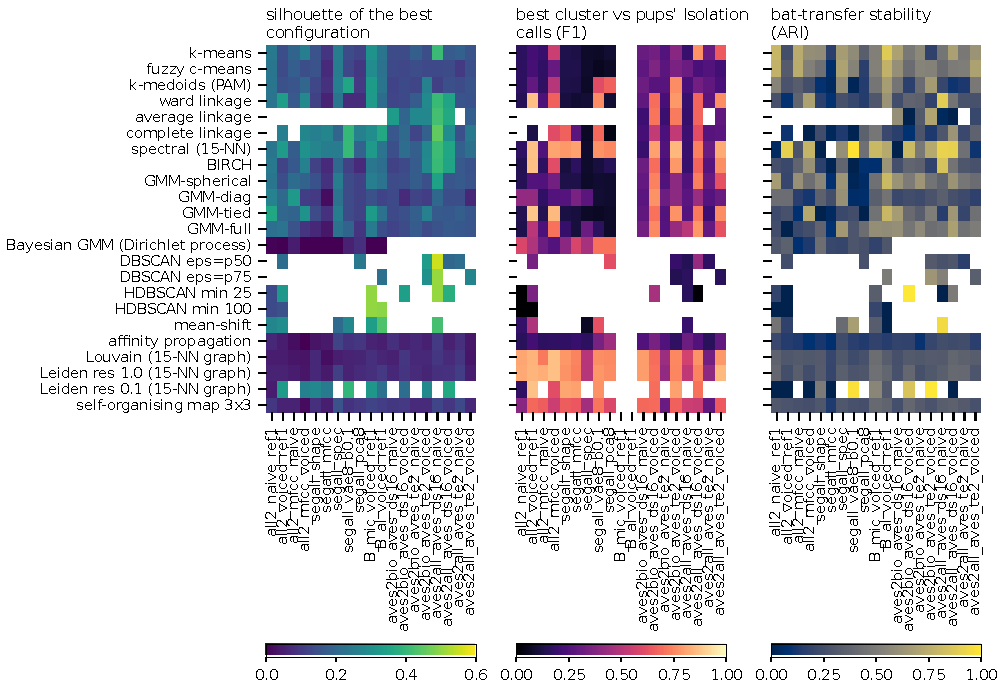
\includegraphics{fig3_v4.pdf}
\caption{\textbf{Figure S7.} Every clustering algorithm on every representation (best configuration with at least two clusters holding $\ge1\%$ of the points; blank = none). Left: silhouette. Middle: F1 of the best cluster for pups' Isolation calls (representations without context labels are blank). Right: bat-transfer stability (adjusted Rand index). Representations are listed in S0; n $\le$ 6,000 points per configuration.}
\end{figure}

\section{Dataset B}
\paragraph{Agreement between sensors.} Independent $k$-means partitions of the same events from the microphone and the piezo agreed beyond chance for the 1,408-statistic features (ARI 0.36--0.44 at $k=2$, 0.20--0.28 at $k=3$--5; for MFCC statistics $-0.01$ to 0.11 at $k=2$ and 0.21--0.31 at $k=3$--5; shuffled-pairing null 0.00) but, within microphone-duration quintiles, the agreement fell to ARI 0.02--0.35: the shared structure is event length and loudness. Sensor agreement is not evidence of biological categories.
\paragraph{Event-level structure.} The microphone's FCM split (FPC 0.629) followed voiced duration (AUC 0.89, \ci{0.86}{0.91}) and SNR (0.90, \ci{0.86}{0.94}); the piezo's followed the same axes (voiced duration AUC 0.86 inverted; SNR 0.82; noise floor 0.83) and was reproducible across individuals (prediction strength 0.93, \ci{0.82}{0.95}; nulls 0.99 and 0.97). The one-cluster battery for the microphone, resampled by individual (five-bat halves), gave prediction strength 0.67 (\ci{0.66}{0.85}; copula null 0.97, session-mean null 0.96), bootstrap Jaccard 0.92 (nulls 0.99, 0.99) and a split-sample dip statistic of 0.0058 within both nulls (0.0078, 0.0052); FPC excess (0.129 against 0.093 and 0.090) and silhouette (0.282 against 0.250 and 0.248) were above the nulls, as in Dataset A, where such excess followed duration and SNR. The piezo's dip statistic (0.0090) exceeded the session-mean null (0.0055; 0 of 50) though not the copula null (0.0090). Event length is multimodal (dip of $\log_{10}$ voiced duration 0.015 for the microphone and 0.012 for the piezo, $p<10^{-4}$; mixture BIC best at $k=3$--5), SNR unimodal.
\paragraph{What these data cannot show.} The events were delimited by the dataset authors' detection pipeline, so the multimodality of event length may be procedural rather than behavioural, and the corpus has no context labels. Individual identity was decoded from the piezo at 0.706 (random folds) and 0.647 (day-blocked) against a 0.227 majority rate and from the microphone at 0.385 and 0.344; because the piezo is attached to each animal, its individual signature may reflect sensor placement. Our energy detector used 10\,dB above the noise floor, chosen so that at least 87\% of events yield voiced frames; the Dataset-A optimum was 20\,dB (F1 0.80).

\section{The June draft}
Audit summary (the full review is in the repository file \texttt{REVIEW\_of\_june\_draft.md}). The 16,000 ``balanced'' calls of the June table are 9,588 distinct annotation rows (948--969 per bat; 39--41\% repeats). Cram\'er's $V$ for emitter $\times$ cluster was 0.457 on all rows ($\chi^2=3{,}339$) and 0.458 on distinct rows ($\chi^2=2{,}009$; bat-level CI \ci{0.21}{0.57}) against a within-strata null of 0.398 (97.5th percentile 0.404); the cluster follows silence (AUC 0.887), span length (0.846) and number of voiced segments (0.852). Its two ``specialist'' bats (88--89\% of calls in the long-file cluster) were both recorded in treatment~9 with median spans of 1.9 and 2.4\,s against 1.3--1.6\,s for the others (Spearman $\rho=-0.90$ across the ten bats between cluster share and median silence, $p=3\times10^{-4}$). Of 45 pairwise Kolmogorov--Smirnov tests, 42 were significant at 0.05 on all rows (39 after Bonferroni correction) and 40 on distinct rows (35 after correction), against 42/45 and 44/45 reported in the two June documents. The robustness table shows that the hard partition is insensitive to the fuzzifier ($m=1.5, 2, 2.5$: ARI 0.983, 0.9995, 0.987; silhouette constant at 0.226; FPC 0.744, 0.584, 0.524), which tests only $m$.

\section{Software, data and reproducibility}
\paragraph{Repository.} [A public repository URL and DOI are to be added by the authors.] The repository holds the analysis scripts (numbered 01--50 in run order), compact per-file feature files (no audio), the merged annotation table, all result tables, figure scripts, the chronological analysis log of every choice and every changed number, and the environment specification.
\paragraph{Environment.} Python 3.13.4 with numpy 2.5.3, scipy 1.18.1, pandas 3.0.6, scikit-learn 1.9.1, statsmodels 0.15.0, librosa 1.0.0, torch 2.14.1, umap-learn 0.5.12, diptest 0.11.0, networkx 3.7, igraph 1.0.0, leidenalg 0.12.0, minisom 2.3.6 and matplotlib 3.11.2; the complete package list is Supplementary Data SD7. The documents were compiled with the Tectonic LaTeX engine.
\paragraph{Execution order.} (1) Sample design and feature extraction from the public archives (scripts 02a, 02, 02b); (2) reproduction of the original matrix (07, 14, 15, 37); (3) analysis sets (05); (4) confound audit and the one-cluster-allowed battery (03a, 03c, 03d, 04, 06, 08); (5) power analysis (22); (6) syllable, VAE and AVES analyses (11, 16, 17, 24, 47); (7) UMAP, HDBSCAN and Isolation-group analyses (12, 21, 23, 26--31, 34, 36, 46); (8) out-of-sample sets (32, 33, 35, 48); (9) all algorithms and sensitivity (20, 38, 41); (10) identity and channel normalisation (18, 19, 25); (11) tables, figures and data export (13, 42--45, 49, 50). Run times are listed in the repository README.
\paragraph{Randomness.} All stochastic steps use seed 42; derived seeds are fixed functions of the seed and the replicate index (for example $42+7919\times$replicate in the power analysis). Scripts 22, 33 and 45 set single-threaded numerical libraries, which affects stored values at the $10^{-5}$ level.
\paragraph{Public and derived data.} Audio comes from the public Dataset A (Prat et al.; Figshare collection doi:10.6084/m9.figshare.c.3666502) and Dataset B (Elie et al.; doi:10.6084/m9.figshare.25886023) and is streamed, not stored. The derived per-file features, the annotation merge and the result tables are shared; the audio is not.
\paragraph{What has been reproduced.} The authors re-ran four analysis scripts (Isolation separability, pair-aware and within-channel identification, confound audit) from the stored features and obtained their stored outputs exactly, and recomputed the display data of the Isolation and replication figures with the original seeds, matching the stored statistics to $10^{-16}$. Extraction of all features from the remote archives was executed once by the authors and has not been independently re-run by another person; a full re-run takes many hours. The extraction code of the original draft analysis is not available, so how its labels were attached to the audio cannot be reproduced; the original matrix itself was reproduced exactly from audio (Table~S0).
\paragraph{Supplementary data files.} SD1, all 1,558 clustering configurations; SD2, the best configuration per algorithm and representation; SD3, power-analysis detection rates with Wilson intervals; SD4, observed and null values of every clusterability statistic; SD5, Isolation AUCs and intervals by age window, channel and treatment; SD6, sample accounting and overlap; SD7, the environment (package list).

\end{document}
